\documentclass{../../slides-style}

\slidetitle{Лекция 3: Scrum}{12.03.2024}

\begin{document}

    \begin{frame}[plain]
        \titlepage
    \end{frame}

    \section{Scrum}

    \begin{frame}
        \frametitle{Scrum}
        \begin{itemize}
            \item Процессный фреймворк для разработки программных продуктов
            \item Не акроним (на самом деле, что-то про командную работу из рэгби)
            \item Ken Schwaber/Jeff Sutherland, 1995 (на самом деле, аж в 1986 году)
            \item Инкрементально-итеративный эмпирический подход
            \begin{itemize}
                \item Источник знаний~--- опыт
            \end{itemize}
            \item Прозрачность, инспекции, адаптация
        \end{itemize}
    \end{frame}

    \section{Роли в команде}

    \begin{frame}
        \frametitle{Роли в команде}
        \begin{columns}
            \begin{column}{0.5\textwidth}
                \begin{itemize}
                    \item Основные 
                    \begin{itemize}
                        \item Product owner
                        \item Scrum master
                        \item Команда разработки
                    \end{itemize}
                \end{itemize}
            \end{column}
            \begin{column}{0.5\textwidth}
                \begin{itemize}
                    \item Вспомогательные 
                    \begin{itemize}
                        \item Пользователи
                        \item Заказчики
                        \item Вспомогательный менеджмент
                        \item Эксперты, консультанты
                    \end{itemize}
                \end{itemize}
            \end{column}
        \end{columns}
        \begin{center}
            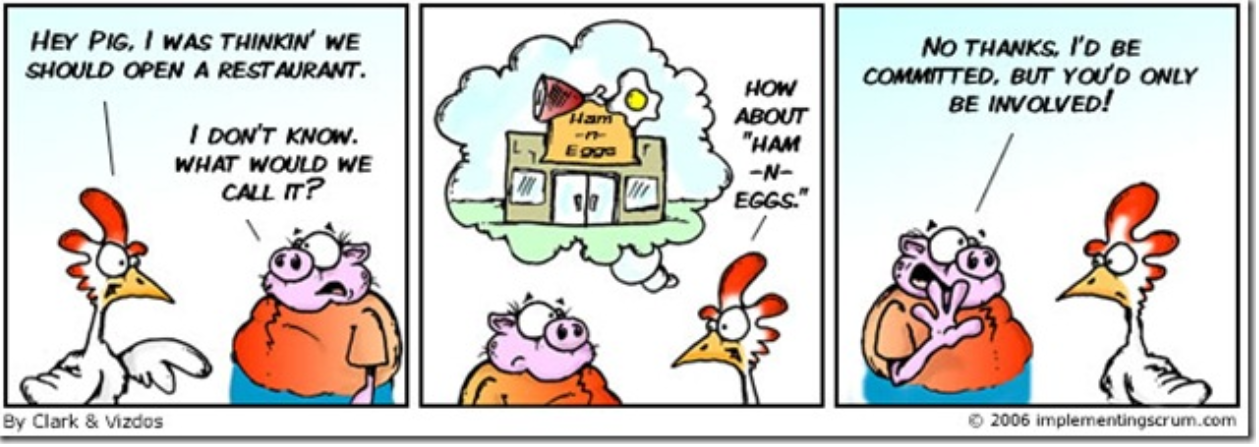
\includegraphics[width=0.8\textwidth]{chickenAndPig.png}
        \end{center}
    \end{frame}

    \begin{frame}
        \frametitle{Product owner}
        \begin{columns}
            \begin{column}{0.7\textwidth}
                \begin{itemize}
                    \item Представляет интересы пользователей
                    \begin{itemize}
                        \item Product manager, project manager, представитель заказчика, \dots
                        \item Заботится о генерации ценности для пользователя
                    \end{itemize}
                    \item Формирует видение проекта и доносит его команде
                    \item Предоставляет требования
                    \item Приоритезирует задачи
                    \item Обеспечивает понятность и ясность задач
                    \item Отвечает за приёмку кода в конце итерации
                    \item Единая точка принятия решений о проекте
                    \begin{itemize}
                        \item Отдельный человек
                    \end{itemize}
                    \item Часть команды, работает у исполнителя
                    \item НЕ начальник
                \end{itemize}
            \end{column}
            \begin{column}{0.3\textwidth}
                \strut
                \begin{center}
                    
\includegraphics[width=0.8\textwidth]{productOwner.png}
                \end{center}
            \end{column}
        \end{columns}
    \end{frame}

    \begin{frame}
        \frametitle{Scrum master}
        \begin{columns}
            \begin{column}{0.7\textwidth}
                \begin{itemize}
                    \item Ответственен за функционирование Scrum-процесса
                    \begin{itemize}
                        \item Следит за соблюдением принципов
                        \item Организует митинги, организует процессы, считает метрики и т.п.
                        \item Разрешает противоречия
                        \item Защищает команду от внешних факторов
                    \end{itemize}
                    \item Лидер-служитель, не имеет особой власти
                    \begin{itemize}
                        \item Коуч, фасилитатор, наставник, тренер, вдохновитель, \dots
                    \end{itemize}
                    \item Помогает команде самоорганизовываться
                    \begin{itemize}
                        \item \emph{Не} управляет командой
                    \end{itemize}
                \end{itemize}
            \end{column}
            \begin{column}{0.3\textwidth}
                \strut
                \begin{center}
                    
\includegraphics[width=0.8\textwidth]{scrumMaster.png}
                \end{center}
            \end{column}
        \end{columns}
    \end{frame}

    \begin{frame}
        \frametitle{Команда разработки}
        \begin{columns}
            \begin{column}{0.7\textwidth}
                \begin{itemize}
                    \item Те, кто на самом деле пишет код
                    \item 7 ± 2 человек
                    \begin{itemize}
                        \item Все в одном месте
                        \item Принцип двух пицц
                    \end{itemize}
                    \item Самоорганизация
                    \item Кроссфункциональность
                    \item Коллективная ответственность
                    \begin{itemize}
                        \item Полный контроль разработки
                    \end{itemize}
                    \item Отсутствие подкоманд
                \end{itemize}
            \end{column}
            \begin{column}{0.3\textwidth}
                \strut
                \begin{center}
                    
\includegraphics[width=0.8\textwidth]{vasyaZemlekop.png}
                \end{center}
            \end{column}
        \end{columns}
    \end{frame}

    \section{Практики}

    \begin{frame}
        \frametitle{Product Backlog}
        \begin{itemize}
            \item Упорядоченный источник всех задач
            \begin{itemize}
                \item Фичи, баги, нефункциональные требования, мероприятия, ...
            \end{itemize}
            \item Единственный источник требований
            \item Ведётся Product owner’ом
            \begin{itemize}
                \item Задачи оцениваются командой
                \item Совместное уточнение задач
            \end{itemize} 
            \item Постоянно пополняется
            \item Единый для нескольких команд
        \end{itemize}
    \end{frame}

    \begin{frame}
        \begin{center}
            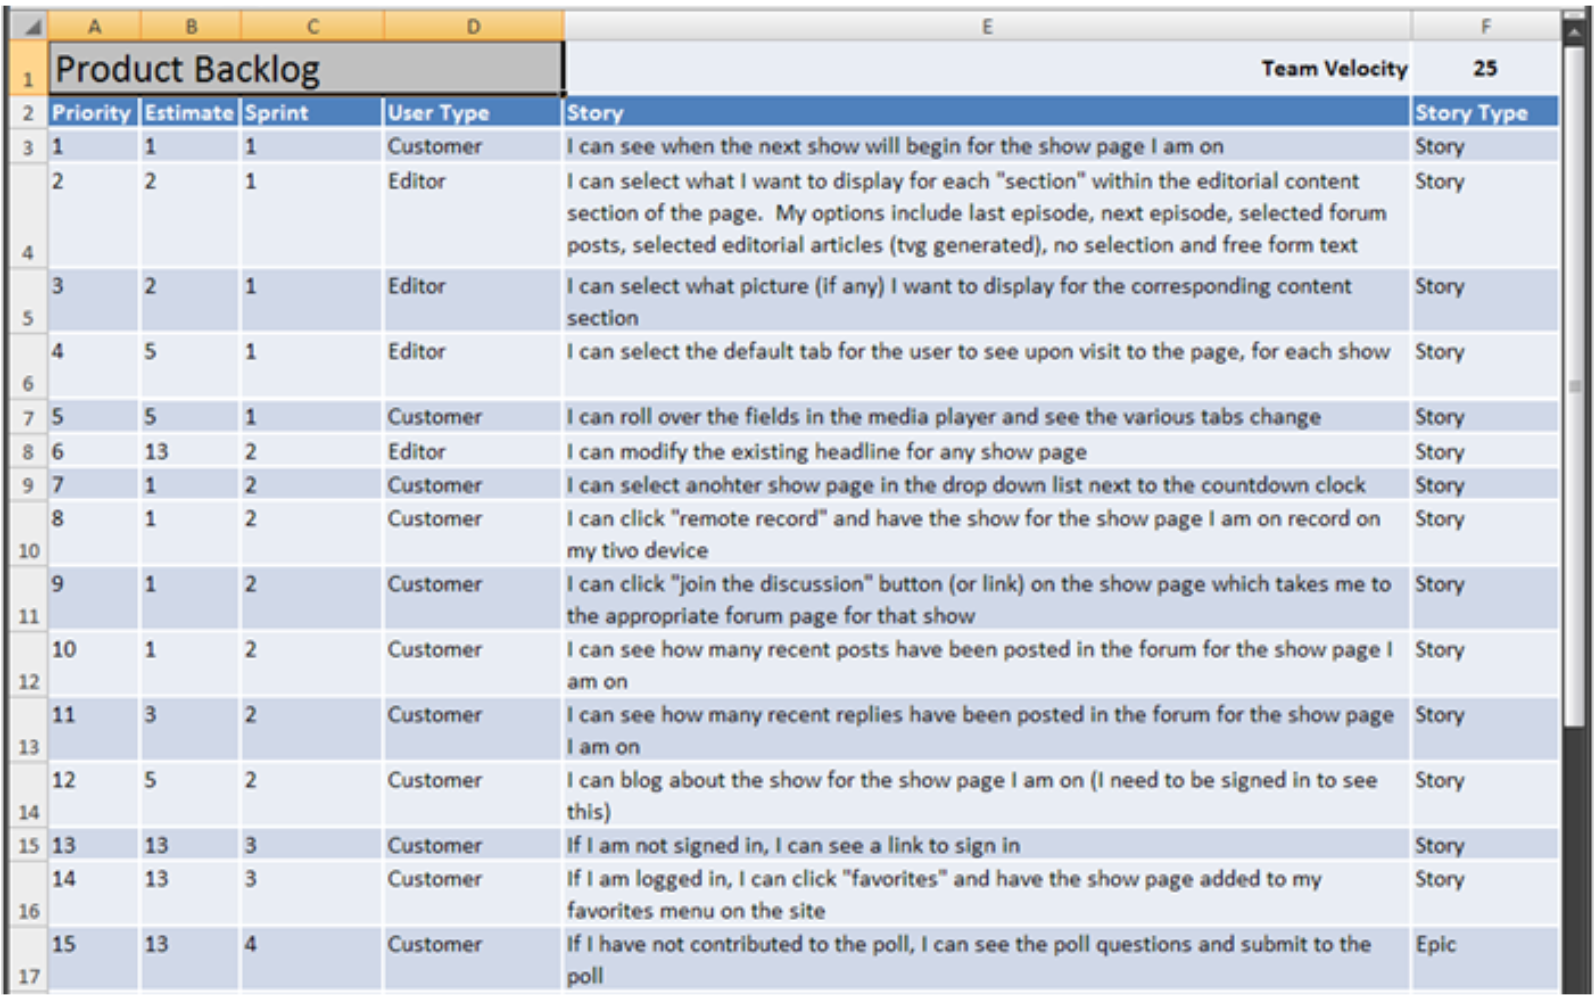
\includegraphics[width=\textwidth]{backlog.png}
        \end{center}
    \end{frame}

    \begin{frame}
        \begin{center}
            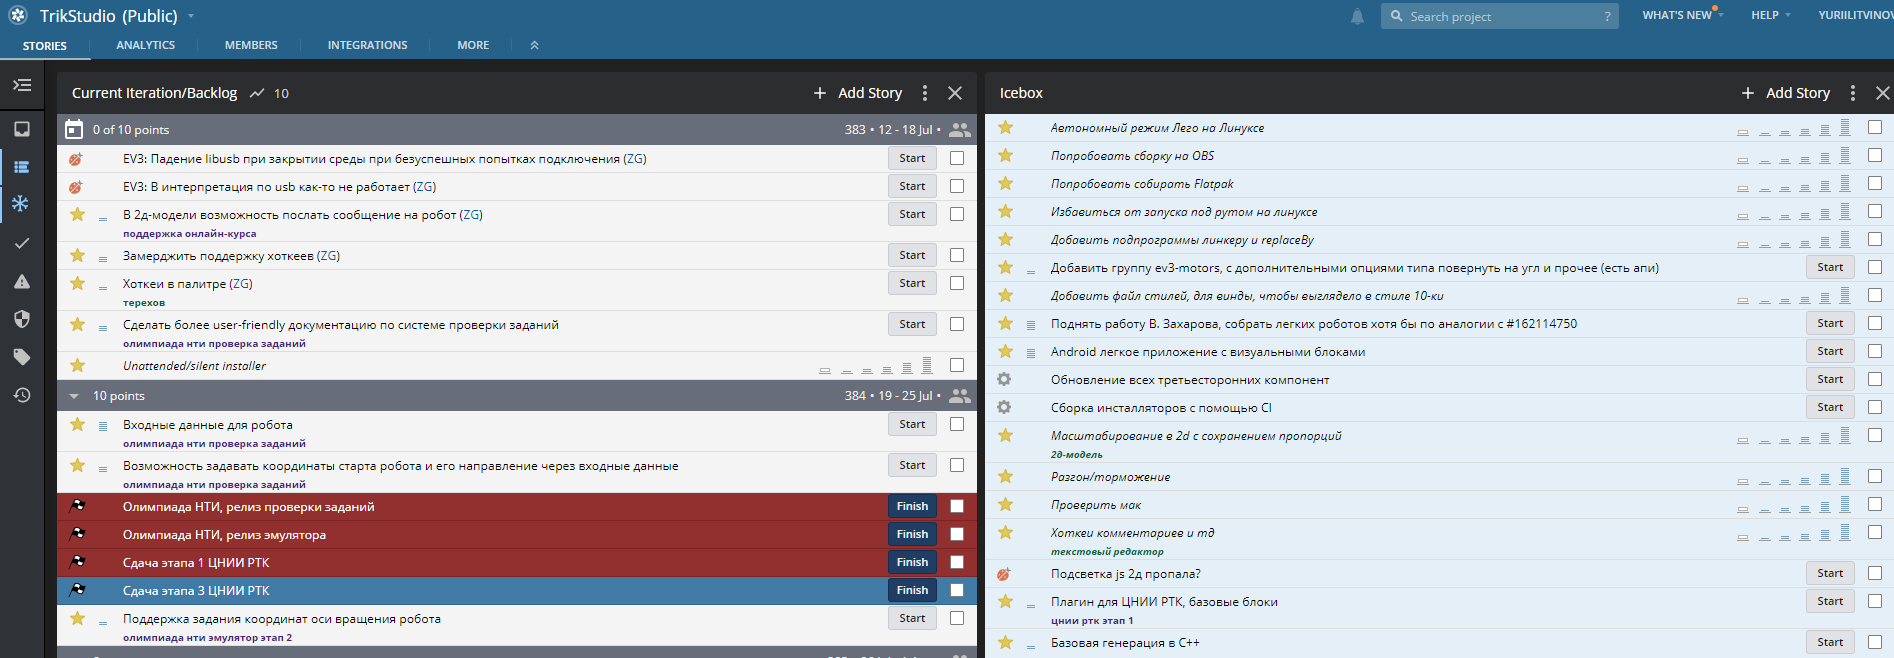
\includegraphics[width=\textwidth]{pivotalTracker.png}
        \end{center}
    \end{frame}

    \begin{frame}
        \frametitle{Спринты}
        \begin{itemize}
            \item Итерация в 1-4 недели
            \item Результат~--- готовая версия (инкремент)
            \begin{itemize}
                \item Или хотя бы что-то осязаемое
            \end{itemize}
            \item Фиксируется объём работ, практически не меняется во время
            спринта
            \item Жизненный цикл спринта
            \begin{itemize}
                \item Планирование
                \item Разработка
                \item Демо
                \item Ретроспектива
            \end{itemize}
        \end{itemize}
    \end{frame}

    \begin{frame}
        \frametitle{Планирование спринта}
        \begin{itemize}
            \item 3-8 часов
            \item Определение целей спринта и набора задач
            \begin{itemize}
                \item Из бизнес-задач формируется sprint backlog
                \item Обычно просто как верхушка Product backlog, которая лезет по
                объёму в спринт
            \end{itemize}
            \item Оценка и упорядочивание задач
            \begin{itemize}
                \item Декомпозиция, добавление технических задач
                \item Planning poker
            \end{itemize}
            \item Коллективная оценка~--- команда не знает, кто какую задачу
            будет делать
            \item Оценка скорости команды (team velocity)
        \end{itemize}
    \end{frame}

    \begin{frame}
        \frametitle{Planning poker}
        \begin{itemize}
            \item Условные единицы, не привязанные напрямую к линейному времени
            \begin{itemize}
                \item team velocity позволяет весьма точно пересчитать в линейный срок
            \end{itemize}
            \item Фибоначчиева шкала (1~--- сейчас сяду и сделаю, держите меня семеро; 8~--- без идей как делать)
            \item Каждый член команды выбирает свою оценку самостоятельно
            \item Потом оценки оглашаются и берётся среднее (почему и покер)
            \item Если есть сильные расхождения, задачу обсуждают, может, декомпозируют, и повторяют голосование
            \item И так по каждой задаче
        \end{itemize}
    \end{frame}

    \begin{frame}
        \begin{center}
            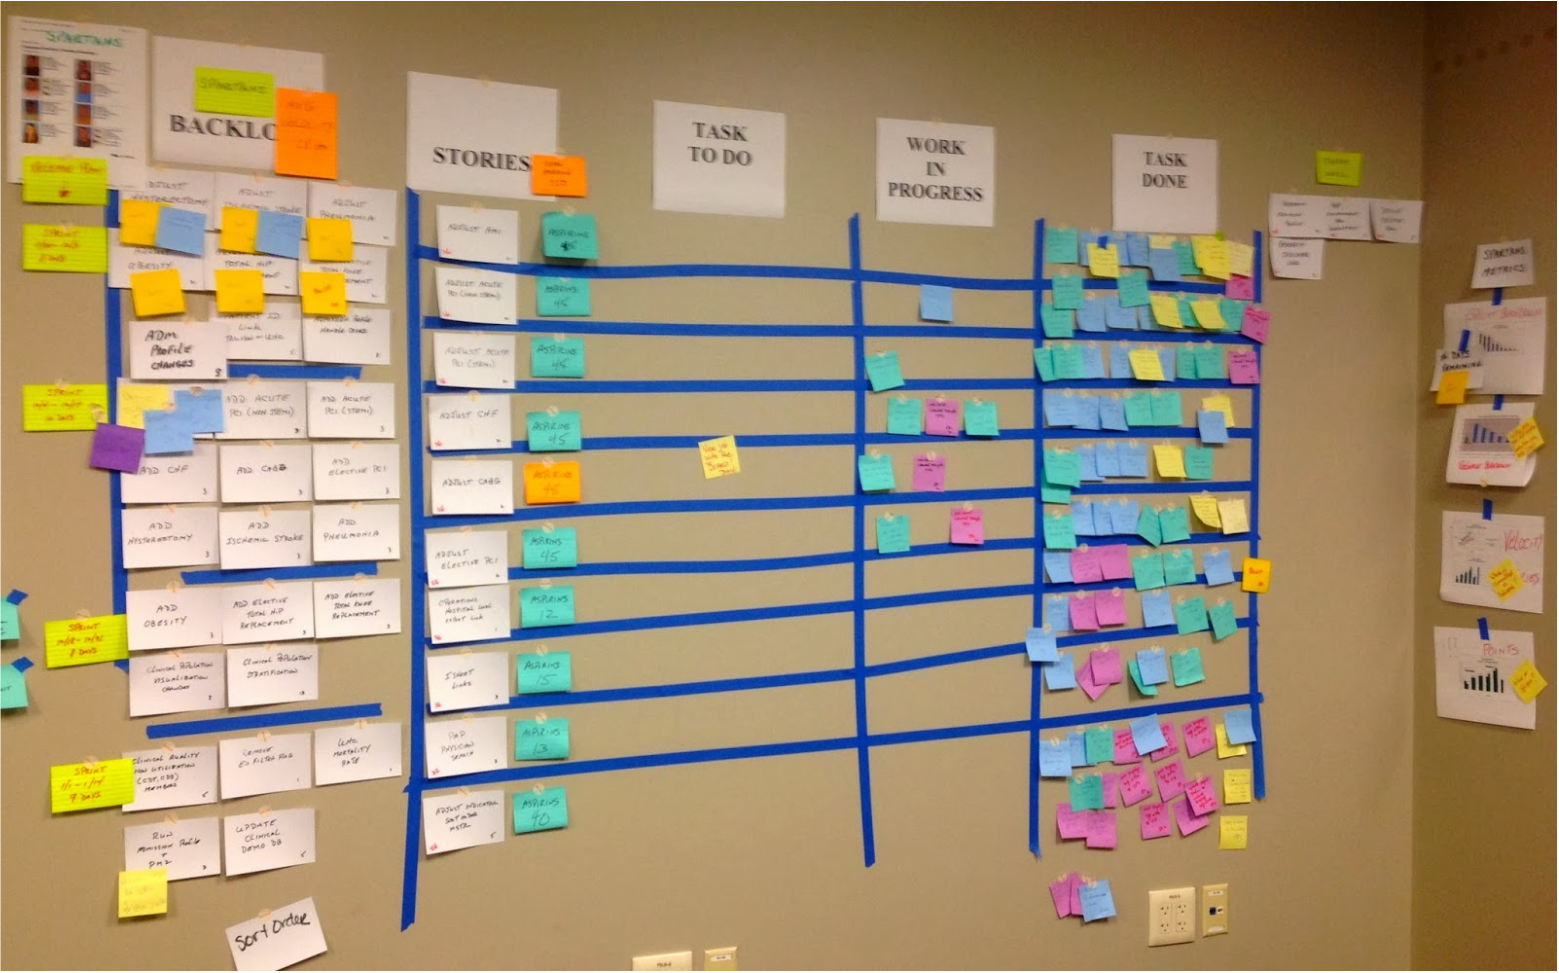
\includegraphics[width=0.8\textwidth]{kanban.png}
        \end{center}
    \end{frame}

    \begin{frame}
        \frametitle{GitHub Projects}
        \begin{center}
            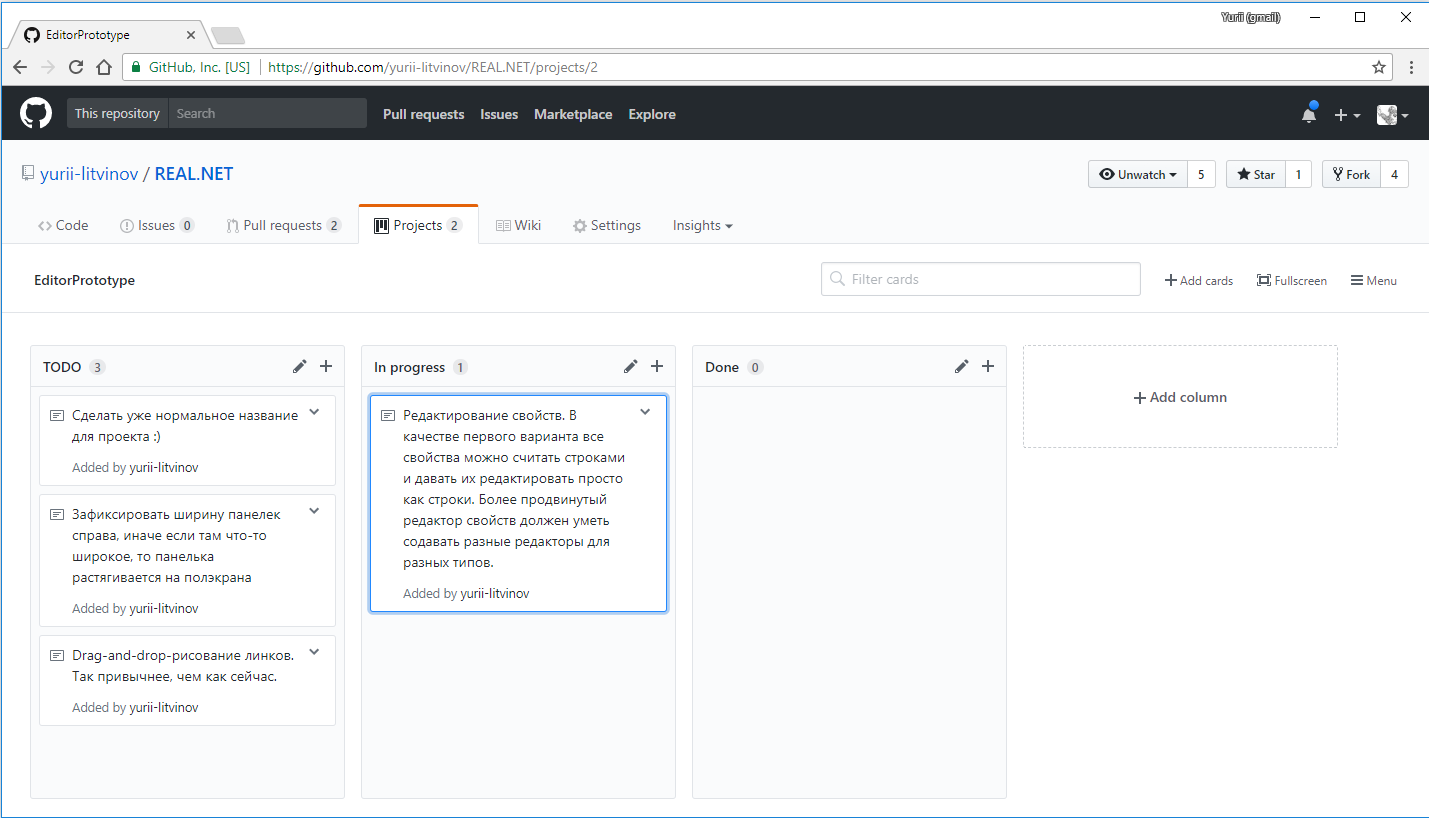
\includegraphics[width=\textwidth]{githubProjects.png}
        \end{center}
    \end{frame}

    \begin{frame}
        \begin{center}
            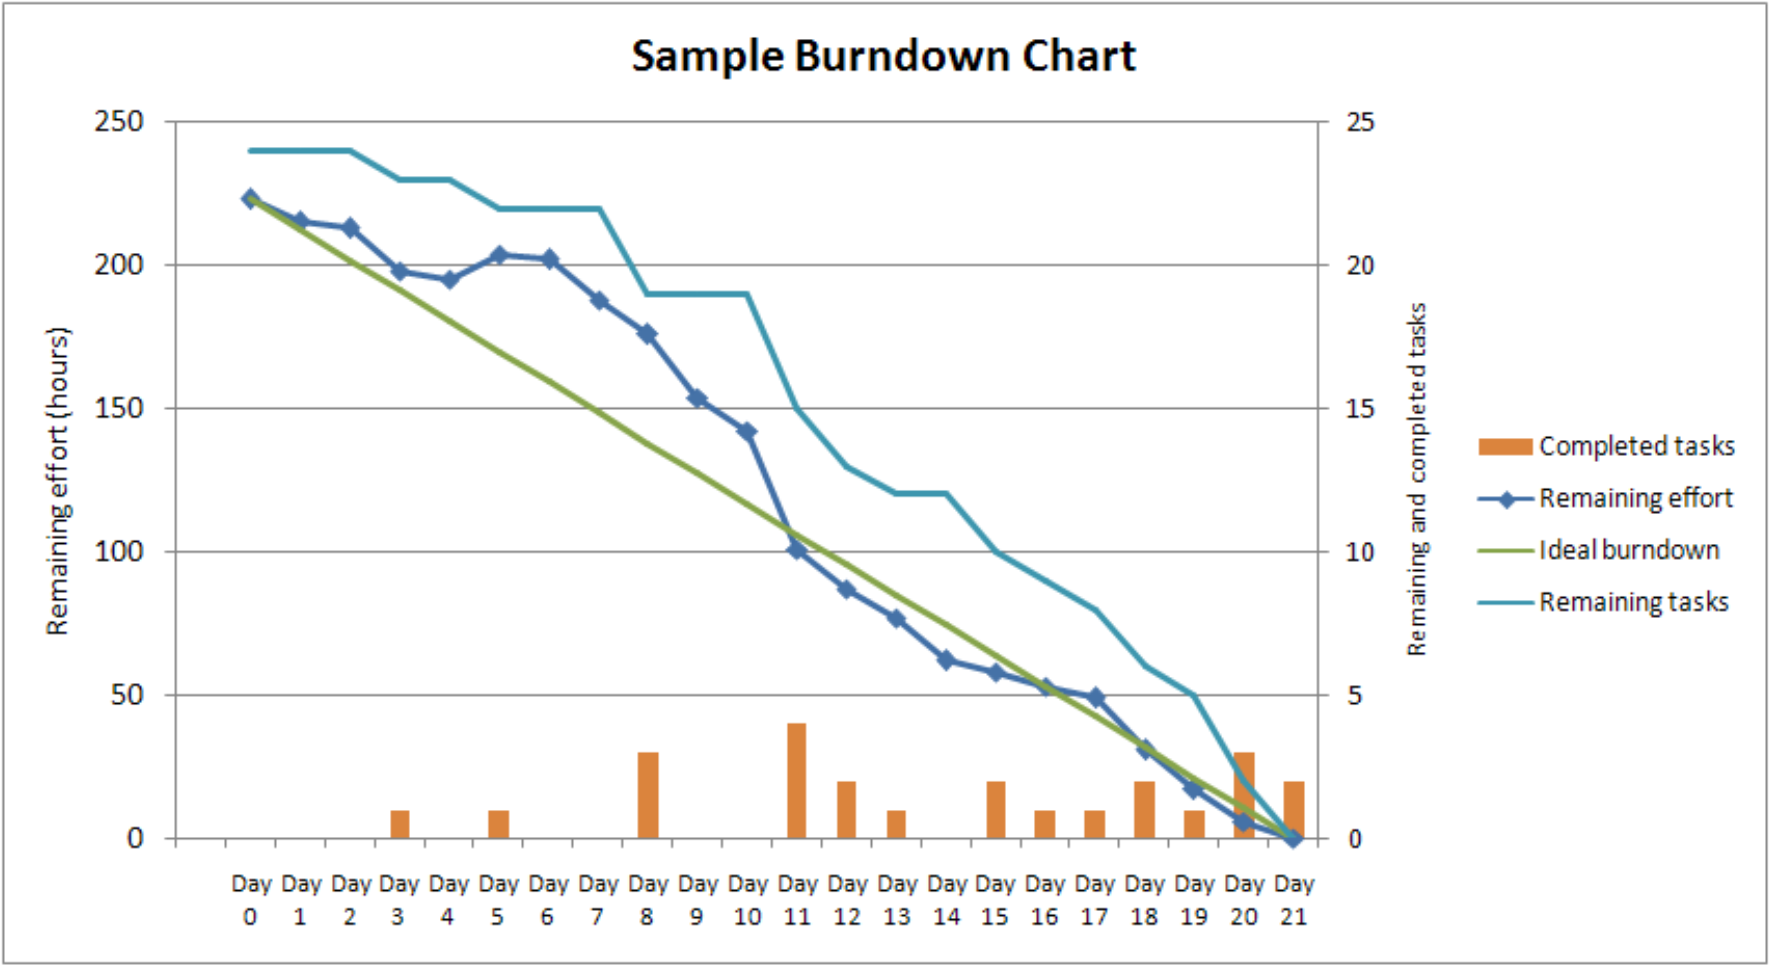
\includegraphics[width=0.8\textwidth]{burndownChart.png}
        \end{center}
    \end{frame}

    \begin{frame}
        \frametitle{Ежедневные встречи}
        \begin{itemize}
            \item Ежедневно, не более 15 минут
            \item Всегда в одно и то же время в одном и том же месте
            \item Участвуют только члены команды разработки
            \item Три вопроса каждому
            \begin{itemize}
                \item Что сделал?
                \item Что буду делать?
                \item Какие есть сложности?
            \end{itemize}
            \item Только делимся информацией, не решаем проблемы
            \item Налаживание связей и распространение информации в команде
            \begin{itemize}
                \item Ключевое мероприятие для инспекции и адаптации
            \end{itemize}
            \item Scrum of Scrums
        \end{itemize}
    \end{frame}

    \begin{frame}
        \frametitle{Ревью спринта/демо}
        \begin{itemize}
            \item Не более 4 часов, в конце спринта
            \begin{itemize}
                \item Плюс подготовка, не более двух часов
            \end{itemize}
            \item Неформальное мероприятие
            \item Демонстрация реализованного инкремента
            \item Обсуждение
            \begin{itemize}
                \item Что делали, что сделали
                \item Что не сделали и почему
                \item Как улучшить процесс далее
            \end{itemize}
            \item Приглашаются все участники проекта
            \begin{itemize}
                \item Обратная связь
            \end{itemize}
            \item Результат~--- обновлённый product backlog
        \end{itemize}
    \end{frame}

    \begin{frame}
        \frametitle{Ретроспектива спринта}
        \begin{itemize}
            \item 1-3 часа, в конце спринта
            \begin{itemize}
                \item После демо и до планирования следующего спринта
            \end{itemize}
            \item Команда разработки и Scrum master
            \item Вопросы:
            \begin{itemize}
                \item Что было сделано хорошо?
                \item что надо улучшить в следующем спринте?
            \end{itemize}
        \end{itemize}
    \end{frame}

    \begin{frame}
        \begin{center}
            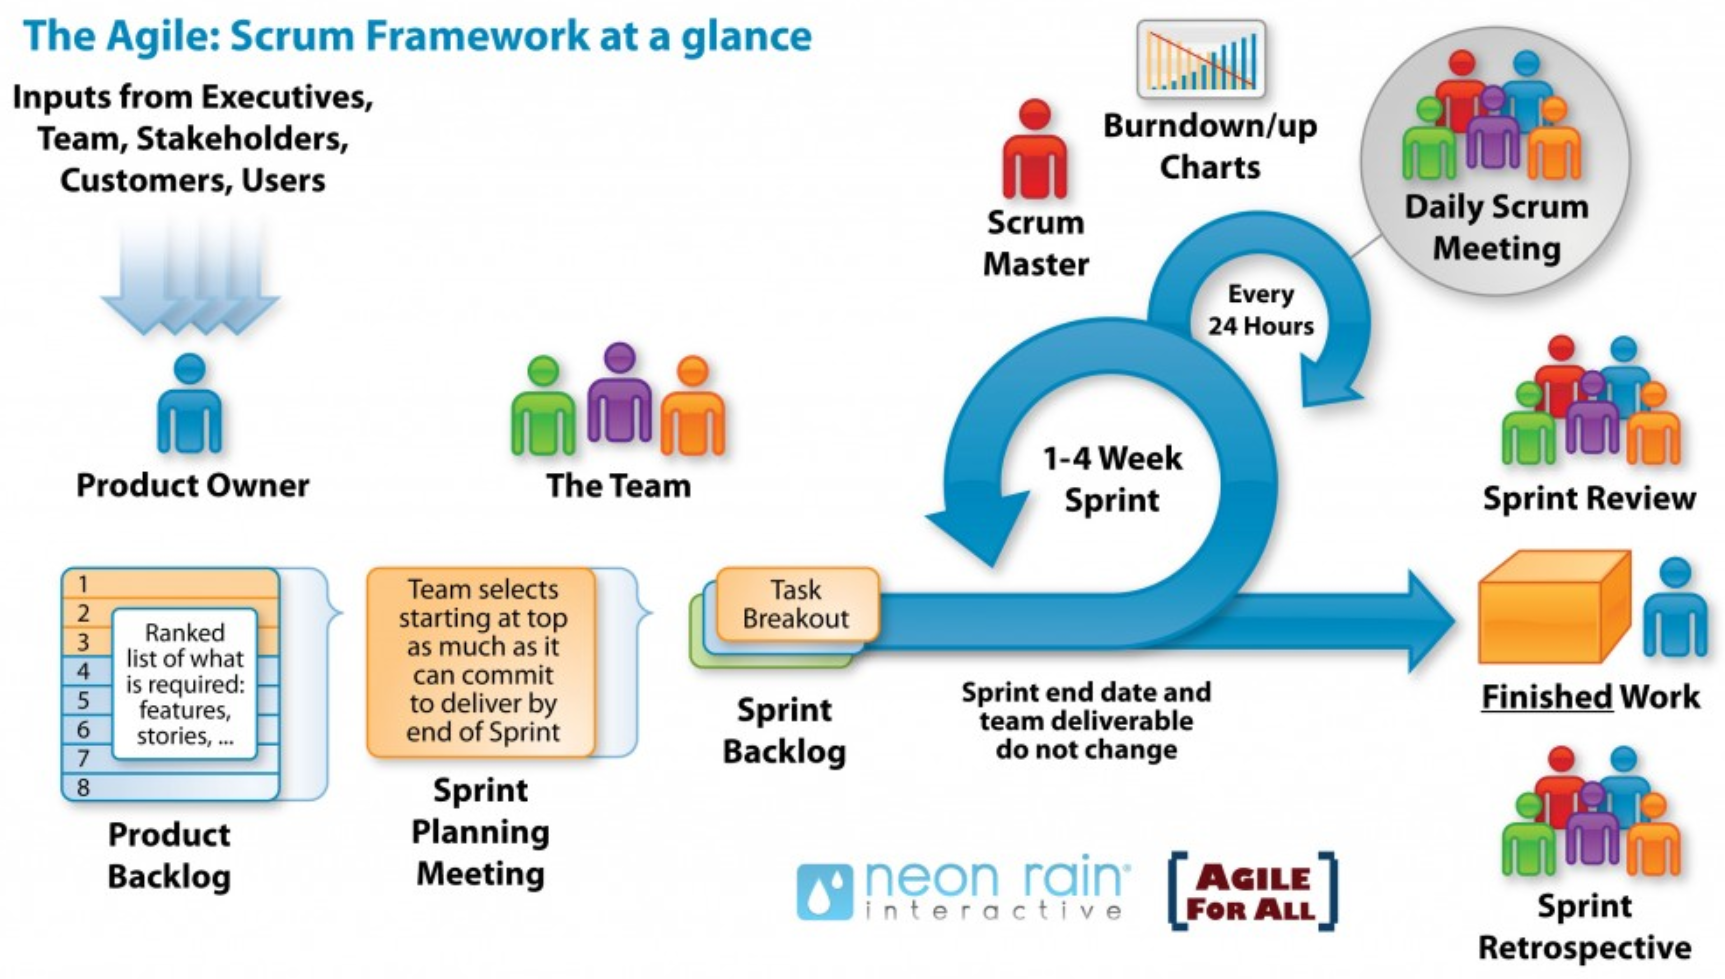
\includegraphics[width=\textwidth]{scrumProcess.png}
        \end{center}
    \end{frame}

    \begin{frame}
        \frametitle{ScrumAnd (Scrum++)}
        \begin{itemize}
            \item Нулевой спринт
            \item Практики XP
            \item Ревью кода
            \item Высокий процент test/code coverage 
            \item All the team testing
            \item Кроссфункциональные работники
            \item Недельные спринты
            \item Широкая аудитория на демо
            \item Автоматизация
        \end{itemize}
    \end{frame}

    \begin{frame}
        \frametitle{ScrumBut (Scrum- -)}
        \begin{itemize}
            \item Персонализация задач/спринтов/багов
            \item ``водопад'' внутри спринта
            \item Ориентация на тулы вместо прямой коммуникации
            \item 6-12-недельные спринты, перерывы между спринтами
            \item Big Design Up-Front (BDUF)
            \item Отсутствие Scrum master’а
            \item Демо по принципу ``Да мы ничего особого не сделали в этом спринте''
            \item Наличие тимлида
        \end{itemize}
        \begin{scriptsize}
            \begin{center}
                \begin{tabularx}{\textwidth} { 
                    | >{\centering\arraybackslash}X 
                    | >{\centering\arraybackslash}X 
                    | >{\centering\arraybackslash}X | }
                    \hline
                    ScrumBut                       & Причина                                           & Решение/Оправдание \\
                    \hline
                    Мы используем Scrum, \emph{НО} & Делать Daily Scrum для нас слишком накладно       & Daily Scrum будет только один раз в неделю               \\
                    \hline
                    Мы используем Scrum, \emph{НО} & Ретроспективы для нас~--- пустая трата времени    & Мы решили их не проводить                                \\
                    \hline
                    Мы используем Scrum, \emph{НО} & Мы не можем доставить инкремент продукта за месяц & Устанавливаем спринт длиной шесть недель                 \\
                    \hline
                    Мы используем Scrum, \emph{НО} & Иногда наши менеджеры дают специальные таски      & Готовые таски не всегда соответствуют Definition Of Done \\
                    \hline
                \end{tabularx}
            \end{center}
        \end{scriptsize}
    \end{frame}

    \begin{frame}
        \frametitle{Принцип Шу-Ха-Ри}
        \begin{center}
            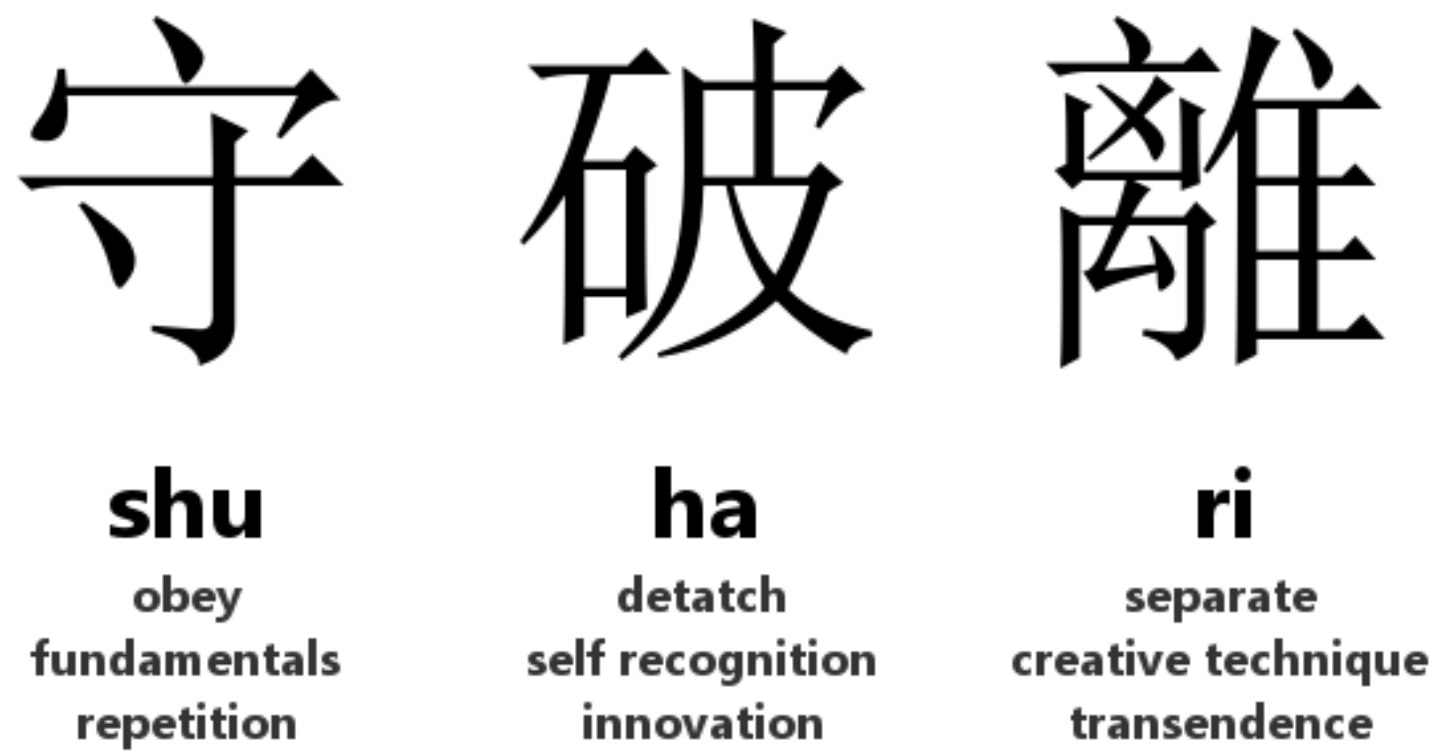
\includegraphics[width=0.9\textwidth]{shuHaRi.png}
        \end{center}
    \end{frame}

    \begin{frame}
        \frametitle{Когда Scrum может работать плохо}
        \begin{itemize}
            \item Fixed-cost/fixed-time проекты
            \item Безответственные, низко мотивированные работники
            \item Слишком узкоспециализированные работники
            \item Неполноставочники
            \item Большое количество внешних зависимостей
            \item Legacy или системы повышенной надёжности
            \item Распределённые команды
            \begin{itemize}
                \item Все более-менее научились работать удалённо
            \end{itemize}
        \end{itemize}
    \end{frame}

    \begin{frame}
        \begin{center}
            
\includegraphics[width=0.6\textwidth]{nextSprint.png}
        \end{center}
    \end{frame}

    \begin{frame}
        \frametitle{Альтенативные подходы к разработке}
        \begin{itemize}
            \item Deadline driven development
            \item Job security driven development
            \item Hate driven development
            \item Hope driven development
            \item Сonference driven development
            \item GitHub Stars driven development
            \item Résumé driven development
        \end{itemize}
    \end{frame}

\end{document}
